\section{An Exemplary 2D Sharp Example}

The example presented here is small enough to describe in full detail and incorporate many of the key features of algebraically correlated random variables described in this work. Presented in two stages, first with sharp inputs replicating an example from Gass \cite{gass75} and the second with algebraically correlated random variable inputs. It will then describe how the example may be generalized.

The basis for the tables and chairs example can be found in Gass \cite{gass75} wherein a decision must be made by a small furniture manufacturer under resource constraints. The choice is whether to manufacture tables or chair or some combination of both. The goal is to maximize the revenue from the sale of the tables and chairs assuming that all will be sold. The specifics are,

\begin{enumerate}
\item There is 400 board-feet of wood available.
\item There is 450 man-hours of labor available.
\item It takes 5 board-feet of wood and 10 man-hours of labor to make a chair.
\item It takes 20 board-feet of wood and 15 man-hours of labor to make a table.
\item Chairs sell for \$45 each.
\item Tables sell for \$80 each.
\end{enumerate}

Stating the problem in standard form according to Boyd \cite{boyd04} and Greenberg \cite{greenberg95},

\begin{align*}
\text{maximize} && 45 x_c + 80 x_t\\
\text{s.t.}     && 5 x_c + 20 x_t \le 400\\
                && 10 x_c + 15 x_t \le 450\\
                && x_c, x_t \ge 0
\end{align*}

where $x_c$ represents the number of chairs to manufacture and sell and $x_t$ represents the number of tables to manufacture and sell.

To form a baseline, first solve this optimization problem using the simplex method as described in the simplex method section. The problem will then be solved again with the prices kept unknown. Random pricing may now be introduced into the problem.

\subsection{Tables and Chairs with All Inputs Sharp and Known}

The simplex method requires all constraints to be stated as equalities so a slack variable introduced into each inequality. The problem is restated as,

\begin{align*}
\text{maximize} && 45 x_c + 80 x_t\\
\text{s.t.}     && 5 x_c + 20 x_t + s_W = 400\\
                && 10 x_c + 15 x_t + s_L\le 450\\
                && x_c, x_t, s_W, s_L \ge 0
\end{align*}

where $s_W$ is the slack variable for the wood resource equation and $s_L$ is the slack variable for the labor resource equation. All variables, $x_c$, $x_t$, $s_W$ and $s_L$ are constrained to be non-negative.

Since each slack variable appears exclusively once in the constraint equations and their coefficients are $+1$ they collectively form a basis for the simplex tableau in table \ref{tab:tc0011}

\begin{table}
\centering
\begin{tabular}{| l | c c c c | c |}
\hline
        & $x_c$ & $x_t$ & $s_W$ & $s_L$ & $b$\\
\hline
$s_W$   & 5     & 20    & 1     & 0     & 400\\
$s_L$   & 10    & 15    & 0     & 1     & 450\\
\hline
Revenue & 45    & 80    & 0     & 0     &\\
\hline
\end{tabular}
  \caption[Tables and Chairs Simplex Tableau for State 0011]
          {Tables and Chairs Simplex Tableau for State 0011}
  \label{tab:tc0011}
\end{table}


The problem variables are collected into the list $X = (x_c, x_t, s_W, s_L)$. Using the order of this list, denote the variables in the current basis with a $1$ and the others with a $0$. The current simplex state is then described with the binary value,

\begin{align*}
State_0 = 0011
\end{align*}

To pivot the table, find the variable to enter the basis and the basis variable to exit the basis. To find the entering variable, compute the cost impact of each,

\begin{align*}
Z_c &= 45 - (5*0 + 10*0) &= 45\\
Z_t &= 80 - (20*0 + 15*0) &= 80
\end{align*}

where $Z_c$ is the cost impact of introducing variable $x_c$ into the basis and $Z_t$ is the cost impact for $x_t$. Recall that increasing $x_c$ the assumed zero value for a non-basis variable by one unit (one more chair sold, for example) will increase revenue by the price of one chair, $\$45$, and will decrease the slack variables $s_W$ and $s_L$ by $5$ and $10$ units respectively. Since there is no revenue impact to increasing or decreasing slack variables the revenue impact is zero for each. 

The entering variable is selected as,
\begin{align*}
\text{argmax}\{Z_c, Z_t\} \implies x_t
\end{align*}

The next simplex state has the form $10??$ because $x_c$ is the entering variable. The question marks indicate that the exiting variable is not yet known.

Since $x_t$ is the entering variable, divide $b = (400, 450)$ element-wise by the basis coefficients for $x_t$ namely $20$ and $15$ and find the minimum non-negative value. In particular one finds,
\begin{align*}
\text{argmin}\{\frac{400}{20}, \frac{450}{15}\} \implies s_W
\end{align*}

Since $\frac{400}{20} < \frac{450}{15}$ and the former value is associated with basis variable $s_W$ it is chosen as the exit variable. Recall that the reason is that the entering variable $x_t$ is allowed to increase from zero and this forces the basis variable in each equation toward zero. In the first equation a unit increase in $x_t$ is a $20$ unit decrease in $s_W = 400$, but only a $15$ unit decrease in $s_L = 450$. Since no variable is allowed to be negative at least one basis variable is driven to zero by an increase in the entering variable. The new simplex state is,
\begin{align*}
State_1 = 0101
\end{align*}

To transform the equations and update the tableau, form the transformation matrix to state $1$,  $B_1$ and its inverse as,
\begin{align*}
B_1 = \begin{pmatrix}20&0\\15&1\end{pmatrix} && B_1^{-1} = \frac{1}{20}\begin{pmatrix}1&0\\-15&20\end{pmatrix}
\end{align*}

recognizing each tableau column as a vector and multiplying on the left by $B_1^{-1}$ creates the new tableau in table \ref{tab:tc0101}.

\begin{table}
\centering
\begin{tabular}{| l | c c c c | c |}
\hline
        & $x_c$ & $x_t$ & $s_W$ & $s_L$ & $b$\\
\hline
$x_t$   & $\frac{1}{4}$     & 1    & $\frac{1}{20}$     & 0     & 20\\
$s_L$   & 6$\frac{1}{4}$    & 0    & -$\frac{3}{4}$     & 1     & 150\\
\hline
Revenue & 45    & 80    & 0     & 0     &\\
\hline
\end{tabular}
  \caption[Tables and Chairs Simplex Tableau for State 0101]
          {Tables and Chairs Simplex Tableau for State 0101}
  \label{tab:tc0101}
\end{table}


The two non-basis variables are now $x_c$ and $s_W$. The cost impact for introducing each into the basis,

\begin{align*}
Z_c &= 45 - (\frac{1}{4}*80 + 6\frac{1}{4}*0) &= 25\\
Z_w &= 0 - (\frac{1}{20}*80 - \frac{3}{4}*0) &= -4 
\end{align*}

where $Z_w$ is the cost impact of (re)-introducing $s_W$ into the basis. Since $Z_w$ is negative, $s_W$ it is not eligible to be a basis vector leaving $x_c$ as the only available choice for entering variable.

Dividing $b$ by the vector of coefficients associated with $x_c$ and finding the smallest non-negative value yields,

\begin{align*}
\text{argmin}\{20 \div \frac{1}{4}, 150 \div 6\frac{1}{4}\} =
\text{argmin}\{80, 24\} \implies s_L
\end{align*}

demonstrating the $s_L$ is the exiting variable. The $B_2$ basis transformation matrix and its inverse become,

\begin{align*}
B_2 = \begin{pmatrix}\frac{1}{4}&1\\6\frac{1}{4}&0\end{pmatrix} && B_2^{-1} = \begin{pmatrix}0&0.16\\1&-0.04\end{pmatrix}
\end{align*}

The simplex state is then,
\begin{align*}
State_2 = 1100
\end{align*}

and the tableau for state 1100 is shown in table \ref{tab:tc1100}.

\begin{table}
\centering
\begin{tabular}{| l | c c c c | c |}
\hline
        & $x_c$ & $x_t$ & $s_W$ & $s_L$ & $b$\\
\hline
$x_c$   & 1    & 0    & -0.12   & 0.16     & 24\\
$x_t$   & 0    & 1    & 0.08    & -0.04    & 14\\
\hline
Revenue & 45    & 80    & 0     & 0     &\\
\hline
\end{tabular}
  \caption[Tables and Chairs Simplex Tableau for State 1100]
          {Tables and Chairs Simplex Tableau for State 1100}
  \label{tab:tc1100}
\end{table}

The two slack variables are no longer in the basis so they are both zero. This means that at the current state all available resources are exhausted to manufacture the tables and chairs. To determine if either of the two slack variables should be re-introduced into the basis, the revenoue impact is calculated for each,

\begin{align*}
Z_W &= 0 - (-0.12*45 + 0.08*80) &= -1\\
Z_L &= 0 - (0.16*45 - 0.04*80) &= -4
\end{align*}

Since each  cost impact is negative there is no possible way to improve the revenue of the problem and the algorithm terminates with the results,

\begin{align*}
x_c &= 24\\
x_t &= 14\\
revenue &= 24*45 + 14*80 = \$2,200
\end{align*}

since $(x_c, x_t) = b$. This means that the optimal choice for the manufacturer is to make 24 chairs and 14 tables which, when sold, will generate a revenue of $\$2,200$.

\begin{figure}
  \centering
  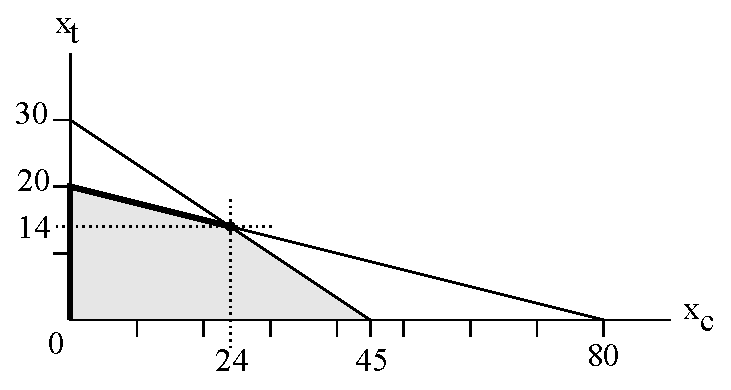
\includegraphics[width=120mm]{Images/tables_and_chairs}
  \caption[Tables and Chairs Constraints and Optimal Point]
          {Tables and Chairs Constraints and Optimal Point}
  \label{fig:tables_and_chairs}
\end{figure}

Figure \ref{fig:tables_and_chairs} shows the resource constraints (diagonal lines), the feasible region (shaded area) and the optimal point, $(24,14)$. The simplex method starts at the origin in this case and follows the heavy line in figure \ref{fig:tables_and_chairs} from vertex to vertex of the polytope described by the half-space constraints to the optimal vertex. Notice that in this case there is an alternate vertex-path from the origin to the optimal vertex, namely passing through point $(45,0)$. The choice of vertex-path is significant as will be seen in the next version of this example when the prices are left unknown.

\subsection{Tables and Chairs with Unknown Prices}

As an intermediate step, consider where uncertainty may be injected into the tables and chairs example. Leaving the prices sharp, but unknown leads to some revealing results.

A priori there are three places in the tables and chairs example where uncertainty may be injected; the constraint vector $b$, the price vector $p$ and the constraint matrix $A$ where,

\begin{align*}
A &= \begin{pmatrix}5&20\\10&15\end{pmatrix}\\
b &= \begin{pmatrix}400\\450\end{pmatrix}\\
p &= \begin{pmatrix}45&80\end{pmatrix}
\end{align*}

Recognize the values in the $A$ matrix as the amount of resources of each type consumed to manufacture each kind of product, $b$ is the number of resources of each kind available and $p$ is the prices charged for each product.

Suppose that instead of the $5$ in matrix $A$, a random variable is introduced. In the context of the tables and chairs example this means that the manufacturer is uncertain about the amount of wood necessary to construct a chair. If there are different kinds of products each would be given separate variables and similarly for each value in the $A$ matrix.

The simplex method uses a \emph{pivot-table} approach whereby a column and related row within the simplex tableau are chosen and a transition is made to a new state within the algorithm. 

The choice of simplex tableau column to replace is made by comparing revenue impacts given a choice of one of the non-basis variables. The values involved in computing the revenue impact of each non-basis variable are prices and products of prices and $A$ matrix coefficients from columns corresponding to the non-basis variables. Assuming that the $A$ matrix values are fixed, linear combinations of $p$ vector prices may be compared to find the  non-basis variable corresponding to the non-negative maximum of revenue impact values.

The choice of simplex tableau row given a column choice is made by finding the quotient of $b$ and the values in $A$ corresponding to that column. Linear combinations of $b$ vector values are compared to find the basis variable corresponding to the the non-negative minimum of linear combinations of constraint values.

Notice that $p$ and $b$ values do not interact directly within the simplex method. Choose the $p$ vector for introduction of random variables suggesting, in the tables and chairs example, price uncertainty over the $b$ vector values which would suggest resource uncertainty. No new insight is gained though choosing $b$ over $p$ or through choosing both for random variable introduction.

In this intermediate tables and chairs example prices $p_c$ and $p_t$ for chairs and tables are unknown, but sharp. Assume the proces are positive. The problem may then be stated in standard form as,

\begin{align*}
\text{maximize} && p_c * x_c + p_t * x_t\\
\text{s.t.}     && 5 x_c + 20 x_t \le 450\\
                && 10 x_c + 15 x_t \le 450\\
                && x_c, x_t \ge 0\\
                && p_c, p_t > 0
\end{align*}

The initial simplex tableau is shown in table \ref{tab:tcp0011}. The only differences from the initial tableau of the first example is the introduction of the state value $0011$ into the upper-left corner and the unknown prices $p_c$ and $p_t$.

\begin{table}
\centering
\begin{tabular}{| l | c c c c | c |}
\hline
0011    & $x_c$ & $x_t$ & $s_W$ & $s_L$ & $b$\\
\hline
$s_W$   & 5     & 20    & 1     & 0     & 400\\
$s_L$   & 10    & 15    & 0     & 1     & 450\\
\hline
Revenue & $p_c$ & $p_t$ & 0     & 0     &\\
\hline
\end{tabular}
  \caption[Tables and Chairs Simplex Tableau for State 0011 with Unknown Prices]
          {Tables and Chairs Simplex Tableau for State 0011 with Unknown Prices}
  \label{tab:tcp0011}
\end{table}

Following the steps from the first example, find the entering non-basis variable by finding,

\begin{align*}
  &\text{argmax}\{p_c - (5*0 + 10*0), p_t - (20*0 + 15*0)\}\\
= &\text{argmax}\{p_c, p_t\}
\end{align*}

Since $p_c, p_t > 0$ neither case may be disqualified there are several possibilities. Either $p_c < p_t$ or $p_c > p_t$ or $p_c = p_t$. Anticipating the introduction, in the next example, of continuous random variables in place of $p_c$ and $p_t$, equality occurs with probability zero so that case is ignored.

If $p_c > p_t$ then choose $x_c$ as the entering variable. To find the exiting variable compute,
\begin{align*}
  &\text{argmin}\{\frac{400}{5}, \frac{450}{10}\}\\
= &\text{argmin}\{80, 45\} \implies s_L
\end{align*}

Since $x_c$ is chosen as the entering variable and $s_L$ as the exiting variable the new state is $1010$ and the transition matrix $B_{1010}$ and its inverse $B_{1010}^{-1}$ is,

\begin{align*}
B_{1010} = \begin{pmatrix}5&1\\10&0\end{pmatrix} && B_{1010}^{-1} = \frac{1}{10}\begin{pmatrix}0&1\\10&-5\end{pmatrix}\end{align*}

The new $1010$ tableau is shown in table \ref{tab:tcp1010}.

\begin{table}
\centering
\begin{tabular}{| l | c c c c | c |}
\hline
1010    & $x_c$ & $x_t$ & $s_W$ & $s_L$ & $b$\\
\hline
$x_c$   & 1     & 1.5    & 0     & 0.1   & 45\\
$s_W$   & 0     & 12.5   & 1     & -0.5  & 175\\
\hline
Revenue & $p_c$ & $p_t$ & 0     & 0     &\\
\hline
\end{tabular}
  \caption[Tables and Chairs Simplex Tableau for State 1010 with Unknown Prices]
          {Tables and Chairs Simplex Tableau for State 1010 with Unknown Prices}
  \label{tab:tcp1010}
\end{table}

The non-basis variables are $x_t$ and $s_L$. Compute the revenue of (re)-introducing each of them, respectively, and find the entering variable,

\begin{align*}
   \text{argmax}\{p_t - (1.5*p_c + 12.5*0), 0 - (0.1*p_c - 0.5*0)\}
= &\text{argmax}\{p_t - 1.5*p_c , - 0.1*p_c\}
\end{align*}

Since $p_c > 0$ then $-0.1*p_c < 0$ so it must be disqualified as an option. The question arises; under what condition is the first options positive? That is,

\begin{align*}
p_t - 1.5*p_c &> 0\\
p_t &> 1.5*p_c\\
\frac{2}{3}p_t &> p_c
\end{align*}

Since it is assumed that $p_c > p_t$ it is not possible for $\frac{2}{3}p_t > p_c$. The simplex algorithm terminates at this point. Since non-basis variables must be zero,

\begin{align*}
x_c &= 45\\
x_t &= 0\\
revenue &= 45p_c && \text{ for } p_t < p_c
\end{align*}

Returning to the first decision point, assume $p_c < p_t$ as was the case in the first example. The tableau under the assumption of transition from state $0011$ to state $0101$ is shown in table \ref{tab:tcp0101}. Notice this is similar to table \ref{tab:tc0101} except for the unknown prices and the state being recorded in the upper left corner of the tableau.

\begin{table}
\centering
\begin{tabular}{| l | c c c c | c |}
\hline
0101    & $x_c$ & $x_t$ & $s_W$ & $s_L$ & $b$\\
\hline
$x_t$   & $\frac{1}{4}$     & 1    & $\frac{1}{20}$     & 0     & 20\\
$s_L$   & 6$\frac{1}{4}$    & 0    & -$\frac{3}{4}$     & 1     & 150\\
\hline
Revenue & $p_c$   & $p_t$    & 0     & 0     &\\
\hline
\end{tabular}
  \caption[Tables and Chairs Simplex Tableau for State 0101 with Unknown Prices]
          {Tables and Chairs Simplex Tableau for State 0101 with Unknown Prices}
  \label{tab:tcp0101}
\end{table}

From state $0101$ the non-basis variables are $x_c$ and $s_W$. Compute the revenue maximizing variables by the usual methods,

\begin{align*}
&\text{argmax}\{p_c - (\frac{1}{4}p_t + 6\frac{1}{4}*0), 0 -
(\frac{1}{20}p_t - \frac{3}{4}*0)\}\\
= &\text{argmax}\{p_c - \frac{1}{4}p_t, -\frac{1}{20}p_t\}
\end{align*}

Since $p_t > 0$ the second option of $-\frac{1}{20}*p_t < 0$ and is disqualified. If $p_c < \frac{1}{4}*p_t$ then the simplex algorithm terminates. The results of this termination are,

\begin{align*}
x_c &= 0\\
x_t &= 20\\
revenue &= 20p_t && \text{ for } p_c < \frac{1}{4}p_t
\end{align*}

For the simplex algorithm to not terminate at this part requires that $p_c > \frac{1}{4}p_t$. Recall that $p_c < p_t$ is assumed at this point. Since these two assumptions are compatible (i.e. not impossible), continue the simplex algorithm. From the calculation for entering variable, notice that $x_c$ is the entering variable and the exiting variable must be found. Recall this situation in the first example and that the result that $s_L$ is the exiting variable and that the resulting tableau is shown in table \ref{tab:tcp1100}. This new figure is nearly identical to the previous table \ref{tab:tc1100}.

\begin{table}
\centering
\begin{tabular}{| l | c c c c | c |}
\hline
1100    & $x_c$ & $x_t$ & $s_W$ & $s_L$ & $b$\\
\hline
$x_c$   & 1    & 0    & -0.12   & 0.16     & 24\\
$x_t$   & 0    & 1    & 0.08    & -0.04    & 14\\
\hline
Revenue & $p_c$ & $p_t$    & 0     & 0     &\\
\hline
\end{tabular}
  \caption[Tables and Chairs Simplex Tableau for State 1100 with Unknown Prices]
          {Tables and Chairs Simplex Tableau for State 1100 with Unknown Prices}
  \label{tab:tcp1100}
\end{table}

Recall that the first example terminated the simplex algorithm upon reaching state (1100). Find the entering variable with the calculation,

\begin{align*}
&\text{argmax}\{0 - (-0.12p_c + 0.08p_t), 0 - (0.16p_c - 0.04p_t)\}\\
= &\text{argmax}\{0.12p_c - 0.08p_t, 0.04p_t - 0.16p_c\}\\
= &\text{argmax}\{3p_c - 2p_t, p_t - 4p_c\}
\end{align*}

For the second option to be positive and therefore available for consideration requires that $p_t > 4p_c$ which is to say $p_c < \frac{1}{4}p_t$. However, to reach this state is was assumed that $p_c > \frac{1}{4}p_t$ so the second option is not available.

If $p_c < \frac{2}{3}p_t$ then the simplex algorithm terminates just as it did in the first example since $45 < \frac{2}{3}*80 = 53.33...$. The result in this case is,

\begin{align*}
x_c &= 14\\
x_t &= 24\\
revenue &= 14p_c + 24p_t && \text{ for } \frac{1}{4}p_t < p_c < \frac{2}{3}p_t
\end{align*}

If $\frac{2}{3}p_t < p_c$ then the first option for the entering variable is available and the entering variable is found to be $s_W$.

The exiting variable in this case is then found as,

\begin{align*}
\text{argmin}\{24 \div -0.12, 14 \div 0.08\}
\end{align*}

Since the first option is negative it is disqualified leaving the second option and therefore the second of the two basis variables $x_t$ as the exiting variable. 

Pivoting on the $s_W$ column and the $x_t$ row results in the transition matrix $B_{1010}$ and its inverse $B_{1010}^{-1}$ as,

\begin{align*}
B_{1010} = \begin{pmatrix}1&-0.12\\0&0.08\end{pmatrix} && 
B_{1010}^{-1} = \begin{pmatrix}1&1.5\\0&125.5\end{pmatrix}
\end{align*}

Applying the transition matrix $B_{1010}^{-1}$ to the $1100$ state tableau return us to the $1010$ state tableau shown in figure \ref{tab:tcp1010}.  State $1010$ terminates so that,

\begin{align*}
x_c &= 45\\
x_t &= 0\\
revenue &= 45p_c && \text{ for } \frac{2}{3}p_t < p_c < p_t
\end{align*}

Since different paths where followed to arrive at state $1010$, the conditions for reaching this state are different. Notice that the conditions for reaching this state directly from the initial $0011$ state are $p_t < p_c$ do not intersect the conditions for reaching this state from state $1010$. Combine the two conditions to see that the revenue outcome of $45p_c$ is reached if $\frac{2}{3}p_t < p_c$.

The result of the investigation is that there are three possible cases for any pair of positive prices given that all other values in the tables and chairs example remain the same, that is,

\begin{align*}
\text{Revenue } = \begin{cases}45p_c & \text{ if } \frac{2}{3}p_t < p_c\\
  24p_c + 14p_t & \text{ if } \frac{1}{4}p_t < p_c < \frac{2}{3}p_t\\
  20p_t & \text{ if } p_c < \frac{1}{4}p_t\end{cases}
\end{align*}

The results of this example are summarized by the directed graph in figure \ref{fig:tc_directed_graph}. The nodes of the graph are the states of the simplex algorithm allied to this example, the edges are marked with the conditions under which the simplex algorithm will follow the edge and the three output cases are labeled $A$, $B$ and $C$ accompanied by the resulting revenue.

\begin{figure}
  \centering
  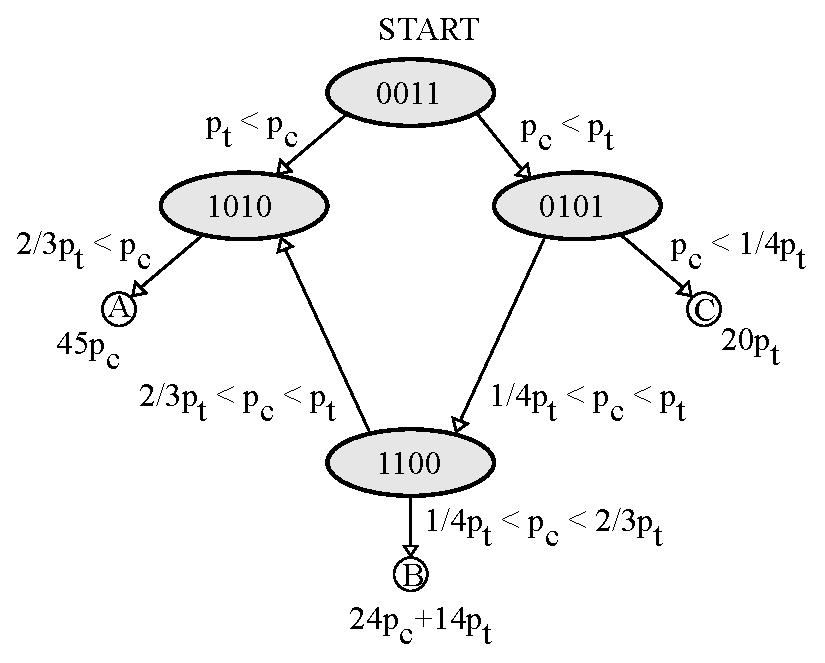
\includegraphics[width=3in]{Images/tc_directed_graph}
  \caption[Tables and Chairs Directed Graph]
          {Tables and Chairs Directed Graph}
  \label{fig:tc_directed_graph}
\end{figure}

Suppose random variables $P_t$ and $P_c$ representing the price of tables and chairs respectively are given. Even if $P_t$ and $P_c$ are correlated in some manner they have a joint distribution which is represetned by the shaded region in figure \ref{fig:tc_joint_prices}. The figure (\ref{fig:tc_joint_prices}) has three levels of shading with each region labeled with its outcome ($A$, $B$ or $C$) corresponding to the directed graph in figure \ref{fig:tc_directed_graph}. Note that if the two price random variables are independent then the shaded region representing the joint probability distribution of $P_t$ and $P_c$ would be rectangular. 

\begin{figure}
  \centering
  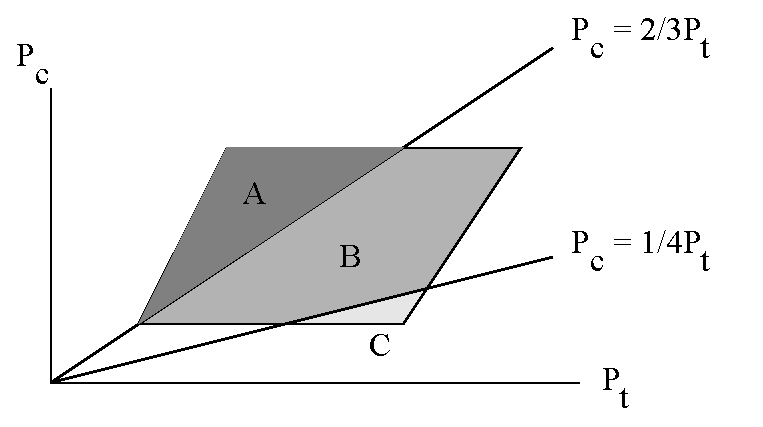
\includegraphics[width=3in]{Images/tc_joint_prices}
  \caption[Tables and Chairs Partitioned Price Probability Space]
          {Tables and Chairs Partitioned Price Probability Space}
  \label{fig:tc_joint_prices}
\end{figure}

